\chapter{Appendix}

\section{Propagators}
\label{app:propagators}

In this Appendix, we derive the classical propagators in superfield notation~\cite{Pawlowski2021}.

The full action of the single-channel model~\eqref{eq:single-channel-action} in position space is~\cite{Boettcher2012}
\begin{align}
    S[\psi, \phi] &= \int_{X,Y} \psi^*_i(Y)
    \left[\left(-\partial_{\tau} - \nabla_X^2 - \mu\right) \delta(X-Y)\right] \psi_i(X) \notag \\
    &+ \int_{X,Y} \phi^*(Y)
    \left[\nu\, \delta(X-Y)\right] \phi(X) \notag \\
    &+ \int_{X,Y,Z} \left[-h \, \delta(Z-X) \delta(Y-X)\right]
	\phi^*(Z) \psi_1(Y) \psi_2(X) \notag \\
	&+ \int_{X,Y,Z} \left[h \, \delta(Z-X) \delta(Y-X)\right]
	\phi(Z) \psi_1^*(Y) \psi_2^*(X) \,.
\end{align}

Defining the Fourier transforms
\begin{align}
    \psi(X) = \int_Q \psi(Q) e^{-iQX} \,, \quad
    \psi^*(X) = \int_Q \psi^*(Q) e^{iQX} \,.
\end{align}

The full action in momentum space is
\begin{align}
    S[\psi, \phi] &= \int_{Q,Q'} \psi^*_i(Q)
    \left[(-i\omega_n + q^2 - \mu) \delta(Q-Q')\right] \psi_i(Q') \notag \\
    &+ \int_{Q,Q'} \phi^*(Q)
    \left[\nu\, \delta(Q-Q')\right] \phi(Q') \notag \\
    &+ \int_{Q,Q',Q''} \left[-h \, \delta\left(Q - (Q'+Q'')\right)\right]
	\phi^*(Q) \psi_1(Q') \psi_2(Q'') \notag \\
	&+ \int_{Q,Q',Q''} \left[h \, \delta\left(Q - (Q'+Q'')\right)\right]
	\phi(Q) \psi_1^*(Q') \psi_2^*(Q'') \,.
\end{align}


In superfield notation~\cite{Pawlowski2021}, we can write the action as
\begin{align}
	\label{eq:superfield-action}
    S[\Phi] &= S^{\psi_i\psi^*_i} \psi^*_i\psi_i + S^{\phi\phi^*} \phi^*\phi
    + S^{\psi_2\psi_1\phi^*} \phi^*\psi_1\psi_2 + S^{\psi^*_2\psi^*_1\phi}
    \phi\psi^*_1\psi^*_2 \,,
\end{align}
where the classical propagators in momentum space are given by
\begin{align}
    S^{\psi_i\psi^*_i} &= \frac{\delta}{\delta\psi_i}\frac{\delta}{\delta\psi^*_i} S[\Phi] 
    = (-i\omega_n + q^2 - \mu) \delta(Q-Q') \,, \notag \\
    S^{\phi\phi^*} &= \frac{\delta}{\delta\phi}\frac{\delta}{\delta\phi^*} S[\Phi]
    = \nu\, \delta(Q-Q') \,, \notag \\
    S^{\psi_2\psi_1\phi^*} &= \frac{\delta}{\delta\psi_2}\frac{\delta}{\delta\psi_1}
    \frac{\delta}{\delta\phi^*} S[\Phi] 
    = -h \, \delta\left(Q - (Q'+Q'')\right) \,, \notag \\
    S^{\psi^*_2\psi^*_1\phi} &= \frac{\delta}{\delta\psi^*_2}\frac{\delta}{\delta\psi^*_1}
    \frac{\delta}{\delta\phi} S[\Phi]
    = h \, \delta\left(Q - (Q'+Q'')\right) \,.
\end{align}
We can also check that the anomalous components are given by
\begin{align}
	S^{\phi\phi} &= \frac{\delta}{\delta\phi}\frac{\delta}{\delta\phi} S[\Phi] = 0 \,, \notag \\
	S^{\phi^*\phi^*} &= \frac{\delta}{\delta\phi^*}\frac{\delta}{\delta\phi^*} S[\Phi] = 0 \,, \notag \\
	S^{\psi_1\psi_2} &= \frac{\delta}{\delta\psi_1}\frac{\delta}{\delta\psi_2} S[\Phi] 
	= h\, \phi^*(Q)\, \delta\left(Q - (Q'+Q'')\right) \,, \notag \\
	S^{\psi^*_2\psi^*_1} &= \frac{\delta}{\delta\psi^*_2}\frac{\delta}{\delta\psi^*_1} S[\Phi]
	= h\, \phi(Q)\, \delta\left(Q - (Q'+Q'')\right) \,.
\end{align}

Note that for fermions and bosons
\begin{align}
    \int_X \psi^*_i(X) \left(\partial_{\tau} - \nabla^2 - \mu\right) \psi_i(X)
    &= \int_X \psi_i(X) \left(\partial_{\tau} + \nabla^2 + \mu\right) \psi^*_i(X) \,, \notag \\
    \int_X \phi^*(X) \left(\partial_{\tau} - \nabla^2 - \mu\right) \phi(X)
    &= \int_X \phi(X) \left(-\partial_{\tau} - \nabla^2 - \mu\right) \phi^*(X) \,,
\end{align}
and therefore the two-point functions satisfy the symmetries
\begin{align}
    S^{\psi^*_i\psi_i}(P) = -S^{\psi_i\psi^*_i}(-P) \,, \qquad
    S^{\phi^*\phi}(P) = S^{\phi\phi^*}(-P) \,,
\end{align}
whereas the three-point function does not contain any derivatives
and is anti-symmetric in the fermionic fields, e.g.,
\begin{align}
    S^{\psi_1\psi_2\phi^*} = -S^{\psi_2\psi_1\phi^*}  \,.
\end{align}

The anomalous propagators satisfy the following symmetries, see also~\cite{Frank2018},
\begin{align}
	S^{\psi_1\psi_2}(P) = S^{\psi^*_2\psi^*_1}(-P)^* \,, \qquad 
	S^{\phi\phi}(P) = S^{\phi^*\phi^*}(-P)^* \,.
\end{align}

\clearpage

\section{Derivation of DSEs}
\label{app:derivation-dse}

In this Appendix, we derive the Dyson-Schwinger equations for the propagators.

The starting point is the general DSE in Eq.~\eqref{eq:DSE-general}, see also~\cite{Pawlowski2021},
\begin{align}
	\frac{\delta\Gamma\left[\Phi\right]}{\delta\Phi_a} =
	\frac{\delta S}{\delta\phi_a}\left[ \phi_b = \Phi_b
	+ G_{bc} \cdot \frac{\delta}{\delta \Phi_c} \right] \,.
\end{align}
Applying this formula to the action~\eqref{eq:superfield-action} in superfield notation yields, e.g., for the fermion propagator
\begin{align}
	\frac{\delta S}{\delta\psi^*_1} = S^{\psi_1\psi^*_1} \psi_1 +
	S^{\psi^*_2\psi^*_1\phi} \phi\psi^*_2 \,.
\end{align}
In terms of the effective fields:
\begin{align}
	\frac{\delta\Gamma}{\delta\Psi_1^*} &=
	S^{\psi_1\psi^*_1} \left[\Psi_1 + G_{\psi_1 k}
	\cdot \frac{\delta}{\delta \Phi_k} \right]
	+ S^{\psi^*_2\psi^*_1\phi} \left[\Phi + G_{\phi l}
	\cdot \frac{\delta}{\delta \Phi_l} \right]
	\left[\Psi^*_2 + G_{\psi^*_2 m}
	\cdot \frac{\delta}{\delta \Phi_m} \right] \notag \\
	&= S^{\psi_1\psi^*_1} \Psi_1 + S^{\psi^*_2\psi^*_1\phi} \Phi \Psi^*_2
	+ S^{\psi^*_2\psi^*_1\phi} G_{\phi \psi^*_2} \,.
\end{align}
Applying another $\delta/\delta\Psi_1$ derivative yields
\begin{align}
	\frac{\delta^2\Gamma}{\delta\Psi_1\delta\Psi_1^*} =
	S^{\psi_1\psi^*_1} + S^{\psi^*_2\psi^*_1\phi}
	\frac{\delta}{\delta\Psi_1} G_{\phi \psi^*_2} \,.
\end{align}
Now, we can use the fact that~\cite{Wink2020}
\begin{align}
	G_{ac} \cdot \Gamma^{cb}
	= (-1)^{ab} \delta^a_b \,,
\end{align}
and therefore~\cite{Pawlowski2021} 
\begin{align}
	\frac{\delta}{\delta\Phi_a} G_{b c}
	= - (-1)^{ab} (-1)^{ee} G_{bd} \cdot \Gamma^{dae} \cdot G_{ec} \,,
\end{align}
to obtain the derivative of the propagator
\begin{align}
	\frac{\delta}{\delta\Psi_1}	G_{\phi \psi^*_2}
	= G_{\phi\phi^*} \cdot \Gamma^{\phi^*\psi_1\psi_2}
	\cdot G_{\psi_2\psi_2^*} \,.
\end{align}
This is a shorthand notation for the full expression
\begin{align}
	\frac{\delta}{\delta\Psi_1(x)}
	G_{\phi \psi_2^*}(y,y)
	= \int_{u,v} G_{\phi\phi^*}(y,u) \,
	\Gamma^{\phi^*\psi_1 \psi_2}(u,x,v) \,
	G_{\psi_2 \psi_2^*}(v,y) \,.
\end{align}
In the end, we arrive at
\begin{align}
	\Gamma^{\psi_1\psi^*_1} = S^{\psi_1\psi^*_1}
	+ S^{\psi^*_2\psi^*_1\phi} \cdot G_{\phi\phi^*}
	\cdot \Gamma^{\phi^*\psi_1\psi_2}
	\cdot G_{\psi_2\psi_2^*}  \,.
\end{align}
This is exactly the DSE which is depicted in the self-energy diagram in Fig.~\ref{fig:prop_DSEs}, after bringing the fields into canonical order and applying the approximation $\Gamma^{\phi^*\psi_1\psi_2} = S^{\phi^*\psi_1\psi_2}$, which gives
\begin{align}
	\Gamma^{\psi_1\psi^*_1} = S^{\psi_1\psi^*_1}
	- S^{\psi^*_2\psi^*_1\phi} \cdot G_{\phi\phi^*}
	\cdot S^{\psi_2\psi_1\phi^*}
	\cdot G_{\psi_2\psi_2^*}  \,.
\end{align}

There will be an overall $\delta(Q-Q')$, so we can write in momentum space
\begin{align}
	\Gamma^{\psi_1\psi^*_1}(P) = S^{\psi_1\psi^*_1}(P)
	+ h^2 \int_Q G_{\phi\phi^*}(Q)
	\cdot G_{\psi_2\psi_2^*}(Q-P)  \,.
\end{align}

\clearpage

The same calculation for the boson propagator:
\begin{align}
	\frac{\delta S}{\delta\phi^*} =
	S^{\phi\phi^*} \phi + S^{\psi_2\psi_1\phi^*} \psi_1 \psi_2 \,.
\end{align}
In terms of the effective fields:
\begin{align}
	\frac{\delta \Gamma}{\delta\Phi^*} &=
	S^{\phi\phi^*} \left[\Phi + G_{\phi k} \cdot
	\frac{\delta}{\delta \Phi_k} \right] + S^{\psi_2\psi_1\phi^*} \left[\Psi_1 +
	G_{\psi_1 l} \cdot \frac{\delta}{\delta \Phi_l} \right]
	\left[\Psi_2 + G_{\psi_2 m}
	\cdot \frac{\delta}{\delta \Phi_m} \right] \notag \\
	&= S^{\phi\phi^*} \Phi + S^{\psi_2\psi_1\phi^*} \Psi_1 \Psi_2
	+ S^{\psi_2\psi_1\phi^*} G_{\psi_1\psi_2} \,.
\end{align}
Applying another $\delta/\delta\Phi$ derivative yields
\begin{align}
	\frac{\delta^2\Gamma}{\delta\Phi\delta\Phi^*} &=
	S^{\phi\phi^*} + S^{\psi_2\psi_1\phi^*} \frac{\delta}{\delta\Phi}
	G_{\psi_1\psi_2} \notag \\
	&= S^{\phi\phi^*} + S^{\psi_2\psi_1\phi^*} \cdot G_{\psi_1\psi_1^*}
	\cdot \Gamma^{\psi_1^*\phi\psi_2^*} \cdot G_{\psi^*_2\psi_2} \,.
\end{align}

Arranging the fields and applying the approximation $\Gamma^{\psi_1^*\phi\psi_2^*} = S^{\psi_1^*\phi\psi_2^*}$ gives
\begin{align}
	\Gamma^{\phi\phi^*} = S^{\phi\phi^*}
	+ S^{\psi_2\psi_1\phi^*} \cdot G_{\psi_1\psi^*_1}
	\cdot S^{\psi_2^*\psi_1^*\phi} \cdot G_{\psi_2\psi^*_2} \,.
\end{align}
In momentum space, this expression reads
\begin{align}
	\Gamma^{\phi\phi^*}(P) = S^{\phi\phi^*}(P)
	- h^2 \int_Q G_{\psi_1\psi^*_1}(Q)
	\cdot G_{\psi_2\psi^*_2}(P-Q) \,.
\end{align}

For completeness, the Dyson-Schwinger equations for the three- and four-point function are depicted in Fig.~\ref{fig:vertex_prop_DSE}.

In the following, we will derive the other equations for the off-diagonal components. See also Ref.~\cite{Haussmann1999,Pieri2004-1}, or Ref.~\cite{Fetter1971} on page 443-446.\\

The other DSE's for the off-diagonal fermionic terms are
\begin{align}
	\Gamma^{\psi_2^*\psi_1^*} &= S^{\psi^*_2\psi^*_1\phi} \phi + S^{\psi^*_2\psi^*_1\phi}
	\frac{\delta}{\delta\Psi_2^*} G_{\phi\psi_2^*} \notag \\
	&= S^{\psi^*_2\psi^*_1\phi} \phi
	+ S^{\psi^*_2\psi^*_1\phi} \cdot G_{\phi\phi} \cdot \Gamma^{\phi\psi^*_2\psi^*_1}
	\cdot G_{\psi^*_1\psi_2^*} \notag \\
	&= \Delta - h^2 \int_Q G_{\phi\phi}(Q)
	\cdot G_{\psi^*_2\psi^*_1}(Q-P) \,,
\end{align}
\begin{align}
	\Gamma^{\psi_1\psi_2} &= - S^{\psi_2\psi_1\phi^*} \phi^* - S^{\psi_2\psi_1\phi^*}
	\frac{\delta}{\delta\Psi_1} G_{\phi^*\psi_1} \notag \\
	&= - S^{\psi_2\psi_1\phi^*} \phi^*
	- S^{\psi_2\psi_1\phi^*} \cdot G_{\phi^*\phi^*} \cdot \Gamma^{\phi^*\psi_1\psi_2}
	\cdot G_{\psi_2\psi_1} \notag \\
	&= \Delta^* - h^2 \int_Q G_{\phi^*\phi^*}(Q)
	\cdot G_{\psi_1\psi_2}(Q-P) \,,
\end{align}

One can see that $\Gamma^{\psi_1\psi_2}(P) = \Gamma^{\psi_2^*\psi_1^*}(-P)^*$ as for the classical two-point functions.

Therefore, one only needs two functions, one normal and one anomalous component.

\clearpage

In the end, we have a fermionic matrix with entries
\begin{align}
	\Gamma^{\Psi\Psi^{\dagger}} =
	\begin{pmatrix}
	\Gamma_{\psi}^{11} & \Gamma_{\psi}^{12} \\
	\Gamma_{\psi}^{21} & \Gamma_{\psi}^{22}
	\end{pmatrix} =
	\begin{pmatrix}
	\Gamma^{\psi_1\psi_1^*} & \Gamma^{\psi_1\psi_2} \\
	\Gamma^{\psi_2^*\psi_1^*} & \Gamma^{\psi_2^*\psi_2}
	\end{pmatrix} \,,
\end{align}
which satisfies
\begin{align}
	G_{\Psi\Psi^{\dagger}} = \left(\Gamma^{\Psi\Psi^{\dagger}}\right)^{-1} \,,
\end{align}
and has entries
\begin{align}
	G_{\Psi\Psi^{\dagger}} =
	\begin{pmatrix}
	G_{\psi_1\psi_1^*} & G_{\psi_1\psi_2} \\
	G_{\psi_2^*\psi_1^*} & G_{\psi_2^*\psi_2}
	\end{pmatrix}
	= \frac{1}{\Gamma_{\psi}^{11}\Gamma_{\psi}^{22}
	-\Gamma_{\psi}^{12}\Gamma_{\psi}^{21}}
	\begin{pmatrix}
	\Gamma_{\psi}^{22} & -\Gamma_{\psi}^{12} \\
	-\Gamma_{\psi}^{21} & \Gamma_{\psi}^{11}
	\end{pmatrix} \,.
\end{align}

More explicitly for the normal fermion propagator, see~\cite{Perali2004, Pieri2004-1},
\begin{align}
	G_{\psi_1\psi_1^*}(Q) = \frac{-S^{\psi_2\psi_2^*}(-Q)+\Sigma_{11}(-Q)}{\left[S^{\psi_1\psi_1^*}(Q)-\Sigma_{11}(Q)\right]
	\left[-S^{\psi_2\psi_2^*}(-Q)+\Sigma_{11}(-Q)\right] - \left[\Gamma^{\psi_1\psi_2}(Q)\right]^2} \,.
\end{align}

One has to be careful with the analytic continuation in the self energy. For $\Sigma_{11}(Q)$ we have it already, but what about $\Sigma_{11}(-Q)$?

For the first case, we had with $i\omega_n \rightarrow \omega + i0^+$:
\begin{align}
	I_{\psi}(\omega,\lambda_1,\lambda_2) = \frac{1}{-\omega + \lambda_1 + \lambda_2}
	+ i \pi \delta(\lambda_1 + \lambda_2 - \omega) \,.
\end{align}

For the case $\Sigma_{11}(-Q)$, we would have
\begin{align}
	I'_{\psi}(\omega,\lambda_1,\lambda_2) = \frac{1}{\omega + \lambda_1 + \lambda_2}
	- i \pi \delta(\lambda_1 + \lambda_2 + \omega) \,.
\end{align}

Thus, it's just $I'(\omega,\lambda_1,\lambda_2) = I(-\omega,\lambda_1,\lambda_2)^*$, as written in~\cite{Pieri2004-1}.


\begin{figure}[b]
	\begin{center}
		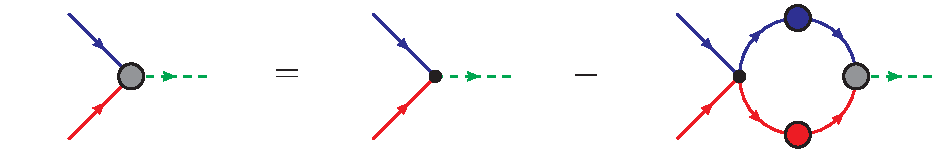
\includegraphics[width=0.7\textwidth]{figs/vertex3_DSE.pdf}\\
		\vspace{0.5cm}
		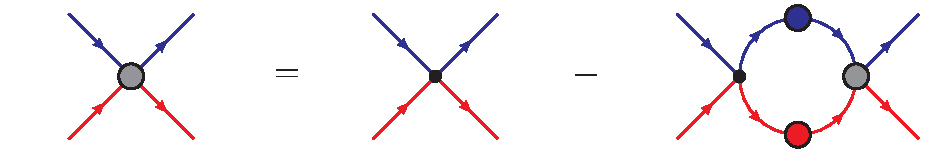
\includegraphics[width=0.7\textwidth]{figs/vertex4_DSE.pdf}
	\end{center}
	\caption[Vertex DSE]{Dyson-Schwinger equation for the three- and four-point function for the full Yukawa theory with background interactions, see~\cite{Diehl2006-1}.}
	\label{fig:vertex_prop_DSE}
\end{figure}


\clearpage

The other DSE's for the off-diagonal bosonic terms are, see Ref.~\cite{Fetter1971} on page 212,
\begin{align}
	\Gamma^{\phi^*\phi^*} &= S^{\psi_2\psi_1\phi^*}
	\frac{\delta}{\delta\Phi^*} G_{\psi_1\psi_2} = S^{\psi_2\psi_1\phi^*}
	\cdot G_{\psi_1\psi_2} \cdot \Gamma^{\psi_2\phi^*\psi_1} \cdot G_{\psi_1\psi_2} \notag \\
	&= h^2 \int_Q G_{\psi_1\psi_2}(Q)\cdot G_{\psi_1\psi_2}(P-Q) \,, \notag \\
	\Gamma^{\phi\phi} &= S^{\psi_2^*\psi_1^*\phi}
	\frac{\delta}{\delta\Phi} G_{\psi_1^*\psi_2^*} = S^{\psi_2^*\psi_1^*\phi}
	\cdot G_{\psi_1^*\psi_2^*} \cdot \Gamma^{\psi_2^*\phi\psi_1^*} \cdot G_{\psi_1^*\psi_2^*} \notag \\
	&= h^2 \int_Q G_{\psi_1^*\psi_2^*}(Q)\cdot G_{\psi_1^*\psi_2^*}(P-Q) \,.
\end{align}

Also in this case, we can see the symmetry $\Gamma^{\phi\phi}(P) = \Gamma^{\phi^*\phi^*}(-P)^*$.

In the end, we have a bosonic matrix with entries
\begin{align}
	\Gamma^{\Phi\Phi^{\dagger}} =
	\begin{pmatrix}
	\Gamma_{\phi}^{11} & \Gamma_{\phi}^{12} \\
	\Gamma_{\phi}^{21} & \Gamma_{\phi}^{22}
	\end{pmatrix} =
	\begin{pmatrix}
	\Gamma^{\phi\phi^*} & \Gamma^{\phi\phi} \\
	\Gamma^{\phi^*\phi^*} & \Gamma^{\phi^*\phi}
	\end{pmatrix} \,,
\end{align}
which satisfies
\begin{align}
	G_{\Phi\Phi^{\dagger}} = \left(\Gamma^{\Phi\Phi^{\dagger}}\right)^{-1} \,,
\end{align}
and has entries
\begin{align}
	G_{\Phi\Phi^{\dagger}} =
	\begin{pmatrix}
	G_{\phi\phi^*} & G_{\phi\phi} \\
	G_{\phi^*\phi^*} & G_{\phi^*\phi}
	\end{pmatrix}
	= \frac{1}{\Gamma_{\phi}^{11}\Gamma_{\phi}^{22}
	-\Gamma_{\phi}^{12}\Gamma_{\phi}^{21}}
	\begin{pmatrix}
	\Gamma_{\phi}^{22} & -\Gamma_{\phi}^{12} \\
	-\Gamma_{\phi}^{21} & \Gamma_{\phi}^{11}
	\end{pmatrix} \,.
\end{align}

For the normal boson propagator, e.g., we have~\cite{Perali2004}
\begin{align}
	G_{\phi\phi^*}(Q) = \frac{\chi_{11}(-Q)}{\chi_{11}(Q)\chi_{11}(-Q)-\chi_{12}(Q)^2} \,,
\end{align}
where $\chi_{11}(Q) = S^{\phi\phi^*}(Q) + \Pi_{11}(Q)$ and $\chi_{12}(Q) = \Pi_{12}(Q)$~\cite{Pieri2004-1}.


\clearpage

\section{Matsubara sums}
\label{app:matsubara-sums}

In this Appendix, we calculate the Matsubara sum in the fermion self-energy, see Eq.~\eqref{eq:spectral-sums},
\begin{align}
	I_{\psi}(\omega_n,\lambda_1,\lambda_2)
	= T \sum_{\Omega_m}
	\frac{1}{i\Omega_m-\lambda_1}
    \frac{1}{i(\Omega_m-\omega_n)-\lambda_2} \,,
\end{align}
where $\Omega_m=2m\pi T$ are bosonic frequencies and $\omega_n=(2n+1)\pi T$
are fermionic~\mbox{frequencies}.

The Bose-Einstein distribution $n_B(z)=1/(e^{\beta z}-1)$ has simple
poles at $z=i\Omega_n$ with residue $1/\beta$, and the Fermi distribution
$n_F(z)=1/(e^{\beta z}+1)$ has simple poles at $z=i\omega_n$ with residue
$-1/\beta$.

The integral along the contour $\mathcal{C}$ over bosonic/fermionic
frequencies $\omega_n$ gives~\cite{Punk2010}
\begin{align}
	T \sum_{\omega_n} h(i\omega_n) =
	\pm \oint_{\mathcal{C}} n_{B/F}(z) h(z) =
	\pm \sum_n
	\mathrm{Res}[n_{B/F}(z) h(z), i\omega_n] \,.
\end{align}
If the function $h(z)$ is analytical on the imaginary axis and vanishes
at infinity, one can deform the contour to exclude the poles on the
imaginary axis and pick up the poles $z_n$ of $h(z)$. Note that the contour
$\mathcal{C}'$ runs clockwise now.
\begin{align}
	T \sum_{\omega_n} h(i\omega_n) =
	\pm \oint_{\mathcal{C}'} n_{B/F}(z) h(z) =
	\mp \sum_n \mathrm{Res}[h(z), z_n] n_{B/F}(z_n) \,.
\end{align}

Applying this to our example above gives
\begin{align}
	I_{\psi}(\omega_n,\lambda_1,\lambda_2)
	&= \oint_{\mathcal{C}'} n_B(z)
	\frac{1}{z-\lambda_1}
    \frac{1}{z-i\omega_n-\lambda_2} \notag \\
    &= \frac{-n_B(\lambda_1)}{-i\omega_n+\lambda_1-\lambda_2} -
    \frac{n_B(i\omega_n+\lambda_2)}{i\omega_n-\lambda_1+\lambda_2} \notag \\
    &= \frac{-n_B(\lambda_1)-n_F(\lambda_2)}{-i\omega_n+\lambda_1-\lambda_2} \,,
\end{align}
where we used $n_B(i\omega_n+z)=-n_F(z)$ for fermionic frequencies in the last line~\cite{Punk2010}.

Analogously for the Matsubara sum in the boson self-energy, see Eq.~\eqref{eq:spectral-sums},
\begin{align}
	I_{\phi}(\omega_n,\lambda_1,\lambda_2)
	= T \sum_{\Omega_m}
	\frac{1}{i\Omega_m-\lambda_1}
    \frac{1}{i(\omega_n-\Omega_m)-\lambda_2} \,,
\end{align}
where now $\Omega_m=(2m+1)\pi T$ are fermionic frequencies and $\omega_n=2n\pi T$
are bosonic~\mbox{frequencies}.
\begin{align}
	I_{\phi}(\omega_n,\lambda_1,\lambda_2)
	&= -\oint_{\mathcal{C}'} n_F(z)
	\frac{1}{z-\lambda_1}
    \frac{1}{i\omega_n-z-\lambda_2} \notag \\
    &= \frac{n_F(\lambda_1)}{i\omega_n-\lambda_1-\lambda_2} -
    \frac{n_F(i\omega_n-\lambda_2)}{i\omega_n-\lambda_1-\lambda_2} \notag \\
    &= \frac{1-n_F(\lambda_1)-n_F(\lambda_2)}{-i\omega_n+\lambda_1+\lambda_2} \,,
\end{align}
where we now used $n_F(i\omega_n+z)=n_F(z)$ for bosonic frequencies. Additionally, we can use the important identities $n_F(-z)=1-n_F(z)$ and $n_B(-z)=-1-n_B(z)$.

\clearpage


\section{Renormalization}
\label{app:renormalization}

In this Appendix, we detail the renormalization procedure and the determination of the model parameters. For more details, see also~\cite{Diehl2006-1,Diehl2008,Punk2010,Schmidt2013}.

The assumption of a pure contact interaction in the single-channel model~\eqref{eq:single-channel-action} leads to unphysical divergences in the theory. In the real world, however, interactions always have a finite range $r_e$ and, thus, a natural momentum cutoff $\Lambda\sim 1/r_e$. In ultracold Fermi gases, the effective range is on the order of the van der Waals length $l_{\mathrm{vdw}}$~\cite{Schmidt2013}. On the other side, one finds that low-energy scattering physics is completely described by the scattering length $a$ and does not depend on the explicit form of the potential. Using this fact, one can regularize the theory and then take the limit of zero range interactions in the end.

We note that the momentum integral in the boson self-energy~\eqref{eq:self-energies} is linearly divergent and needs regularization. This is provided by the renormalization of $\nu$, which will cure all divergences of the theory. The physical renormalization condition is given by the connection to the two-body scattering length $a$ in vacuum~\cite{Schmidt2011,Frank2018-1}. The scattering of two fermions is mediated by the exchange of the bosonic dimer $\phi$. Evaluating the tree-level diagram for the effective fermion-fermion scattering in Fig.~\ref{fig:two-body-scattering} shows that the scattering amplitude $f(k)$ is related to the full boson propagator $G_{\phi}$ via~\cite{Schmidt2011,Zwerger2016}
%
\begin{align}
	\label{eq:scattering-amplitude-propagator}
	f(k) = \frac{h^2}{8\pi} G_{\phi}(2k^2,\bm{0}) \,,
\end{align}
%
where $E=2k^2$ is the total energy in the center of mass frame of incoming fermions with momenta $k$. This expression should be equal to the well-known result from low-energy s-wave scattering theory with zero effective range~\cite{Frank2018-1,Schmidt2013}
%
\begin{align}
	f(k) = \frac{1}{-1/a-ik} \,.
\end{align}
%
Thus, the renormalization condition for two-body scattering in vacuum is
%
\begin{align}
	G_{\phi}(0,\bm{0}) = -\frac{8\pi a}{h^2} \,.
\end{align}
%
This can be written in terms of the bare detuning $\nu$,
%
\begin{align}
	\nu = -\frac{h^2}{8\pi a} + \tilde{\Pi}_{\phi}(0,\bm{0}) \,,
\end{align}
%
where $\tilde{\Pi}_{\phi}$ is the bare boson self-energy. Thus, the renormalized boson DSE is
%
\begin{align}
	\Gamma^{(2)}_{\phi\phi^*}(\omega,\bm{p}) &= -\frac{h^2}{8\pi a} - \left[ \tilde{\Pi}_{\phi}(\omega,\bm{p}) - \tilde{\Pi}_{\phi}(0,\bm{0}) \right] \,.
\end{align}
%

\begin{figure}[h]
	\centering
	
\includegraphics[width=0.55\textwidth]{figs/two-body.pdf}
	\caption[Two-body scattering]{Tree-level diagram yielding the effective two-body scattering amplitude.}
	\label{fig:two-body-scattering}
\end{figure}

The renormalized boson self-energy $\Pi_{\phi}(\omega,\bm{p})=\tilde{\Pi}_{\phi}(\omega,\bm{p}) - \tilde{\Pi}_{\phi}(0,\bm{0})$, which also appears in Eq.~\eqref{eq:selfconsistent-equations}, is finite due to the counterterm $\tilde{\Pi}_{\phi}(0,\bm{0})$. To determine this counterterm, one has to consider the two-body problem in vacuum, i.e. $T=\mu=0$. In this case, the full boson self-energy can be solved exactly~\cite{Diehl2006-1,Schmidt2013}, since the fermions are not dressed. Evaluating the self-energy loop integral with the bare fermion propagators yields
%
\begin{align}
	\tilde{\Pi}_{\phi}(0,\bm{0}) &= h^2 \int_{\bm{q}}^{\Lambda} \frac{1}{2\varepsilon_{\bm{q}}} = \frac{h^2\Lambda}{4\pi^2} \,,
\end{align}
%
where $\Lambda$ is the aforementioned momentum cutoff that regularizes the integral. This counterterm cures all linear divergences arising from the contact interaction and allows to take the limit of $\Lambda$ to infinity in the end. For example, the renormalized boson self-energy in vacuum is then
%
\begin{align}
	\Pi_{\phi}(\omega, \bm{p}) &= h^2 \int_{\bm{q}}^{\Lambda} \left[\frac{1}{-\omega+\varepsilon_{\bm{q}}+\varepsilon_{\bm{p-q}}-i0^+} - \frac{1}{2\varepsilon_{\bm{q}}}\right] \notag \\
	&= \frac{h^2}{8\pi} \sqrt{-\frac{\omega}{2}+\frac{\bm{p}^2}{4}-i0^+}  \,,
\end{align}
%
with $\Lambda\rightarrow\infty$. For this reason, we can formally write the bare detuning $\nu$ as~\cite{Haussmann2009,Zwerger2016}
%
\begin{align}
	\label{eq:renorm-detuning}
	\nu = -\frac{h^2}{8\pi a} + \int_{\bm{q}} \frac{1}{2\varepsilon_{\bm{q}}} \,.
\end{align}



\clearpage

%%%%%%%%%%%%%%%%%%%%%%%%%%%%
\section{Boson self-energy calculation}
\label{app:boson-self-energy-calculation}

In this Appendix, we show the explicit computations and analytic results for the boson self-energy with general spin and mass-imbalance. Throughout this part, we use the same notation as introduced in Section~\ref{section:polaron-theoretical-description}. We start from the general expression for the non-selfconsistent boson self-energy with mass-imbalance $\alpha$,
\begin{align}
	\Pi_{\phi}(\omega_n, \bm{p}) =
	h^2 \int_{\bm{q}} \left[ T\sum_{\Omega_m}
	G^{(0)}_{\downarrow}(\Omega_m, \bm{q})
	G^{(0)}_{\uparrow}(\omega_n-\Omega_m, \bm{p-q}) - \frac{1+\alpha}{2\bm{q}^2} \right] \,.
\end{align}
Inserting the classical fermion spectral functions, we obtain the well-known result
\begin{align}
	\Pi_{\phi}(\omega_n, \bm{p}) &= h^2 \int_{\bm{q}} \left[ T\sum_{\Omega_m}
	\frac{1}{i\Omega_m-\varepsilon^{(I)}_{\bm{q}}+\mu_{\downarrow}}
	\frac{1}{i(\omega_n-\Omega_m)-\varepsilon_{\bm{p-q}}+\mu_{\uparrow}} - \frac{1+\alpha}{2\bm{q}^2} \right] \notag \\
	&= h^2 \int_{\bm{q}} \left[ \frac{1-n_F(\varepsilon^{(I)}_{\bm{q}}-\mu_{\downarrow}) -  n_F(\varepsilon_{\bm{p-q}}-\mu_{\uparrow})}{-i\omega_n+\varepsilon^{(I)}_{\bm{q}}+\varepsilon_{\bm{p-q}}-\mu_{\downarrow}-\mu_{\uparrow}} - \frac{1+\alpha}{2\bm{q}^2} \right] \,,
\end{align}
where $\varepsilon^{(I)}_{\bm{p}}=\bm{p}^2\,(1-\alpha)/(1+\alpha)$. From here, one can obtain the real and imaginary part of the retarded self-energy $\Pi_{\phi}^R(\omega,\bm{p})$ after analytic continuation $i\omega_n\rightarrow\omega+i0^+$. It is useful to separate the boson self-energy into a vacuum part and a temperature-dependent part, $\Pi^{R}_{\phi} = \Pi^{R,0}_{\phi} + \Pi^{R,T}_{\phi}$, where the vacuum part is given by
\begin{align}
	\Pi^{R,0}_{\phi}(\omega, \bm{p}) =
	h^2 \int_{\bm{q}} \left[ \frac{1}{-\omega+\varepsilon^{(I)}_{\bm{q}}+\varepsilon_{\bm{p-q}}-\mu_{\downarrow}-\mu_{\uparrow}-i0^+} - \frac{1+\alpha}{2\bm{q}^2} \right] \,,
\end{align}
Performing the variable shift $\bm{q} \rightarrow \bm{q} + (1+\alpha)\bm{p}/2$ makes the angle integration trivial and we obtain further for the vacuum part
\begin{align}
	\Pi^{R,0}_{\phi}(\omega, \bm{p}) =
	\frac{h^2(1+\alpha)}{4\pi^2} \int_0^{\infty} dq \left[\frac{q^2}{q^2-y-i0^+}-1\right]
	= \frac{h^2(1+\alpha)}{8\pi} \sqrt{-y-i0^+} \,,
\end{align}
where we have defined
\begin{align}
	y = \frac{(1+\alpha)}{2}
	\left[\omega-\frac{(1-\alpha)}{2}p^2
	+\mu_{\uparrow}+\mu_{\downarrow}\right] \,.
\end{align}

The temperature-dependent part can be divided into the $\downarrow$ and $\uparrow$ contribution and is obtained by the same means
\begin{align}
	\Pi^{R,T}_{\phi,\downarrow}(\omega, \bm{p}) = -
	\frac{h^2(1+\alpha)}{4\pi^2} \int_0^{\infty}
	\frac{\chi_{\downarrow}(q) \, q^2 \, dq}{q^2-y-i0^+} \,,
\end{align}
\begin{align}
	\Pi^{R,T}_{\phi,\uparrow}(\omega, \bm{p}) = -
	\frac{h^2(1+\alpha)}{4\pi^2} \int_0^{\infty}
	\frac{\chi_{\uparrow}(q) \, q^2 \, dq}{q^2-y-i0^+} \,,
\end{align}
where we have defined the two angle-integrated functions $\chi_{\downarrow}(q)$ and $\chi_{\uparrow}(q)$.

The angle-integrated functions at finite temperature are given by
\begin{align}
	\chi_{\downarrow}(q) &= \int_{-1}^1 \frac{dx}{2} \,
	n_F\left(\frac{(1-\alpha)}{(1+\alpha)}
	\left[\bm{q}+(1+\alpha)\bm{p}/2\right]^2
	-\mu_{\downarrow}\right) \notag \\
	&=
	\begin{cases}
		n_F\left(\frac{(1-\alpha)}{(1+\alpha)}
		q^2-\mu_{\downarrow}\right) & ,\, \bm{p} = \bm{0} \\
		\frac{T}{2(1-\alpha)pq} \ln\left( \frac{
			n_F\left(\mu_{\downarrow}-\frac{(1-\alpha)}{(1+\alpha)}
			\left[q+(1+\alpha)p/2\right]^2\right)}{
			n_F\left(\mu_{\downarrow}-\frac{(1-\alpha)}{(1+\alpha)}
			\left[q-(1+\alpha)p/2\right]^2\right)}
		\right) & ,\, \bm{p} \neq \bm{0}
	\end{cases} \,,
\end{align}
\begin{align}
	\chi_{\uparrow}(q) &= \int_{-1}^1 \frac{dx}{2} \,
	n_F\left(\left[\bm{q}-(1-\alpha)\bm{p}/2\right]^2
	-\mu_{\uparrow}\right) \notag \\
	&=
	\begin{cases}
		n_F\left(q^2-\mu_{\uparrow}\right) & ,\, \bm{p} = \bm{0} \\
		\frac{T}{2(1-\alpha)pq} \ln\left( \frac{
			n_F\left(\mu_{\uparrow}-\left[q+(1-\alpha)p/2\right]^2\right)}{
			n_F\left(\mu_{\uparrow}-\left[q-(1-\alpha)p/2\right]^2\right)}
		\right) & ,\, \bm{p} \neq \bm{0}
	\end{cases} \,.
\end{align}
Here, $x=\cos(\theta_{\bm{pq}})$ and $\theta_{\bm{pq}}$ is the angle between the vectors $\bm{p}$ and $\bm{q}$. Note that these functions leaves a non-zero contribution in the vacuum for $\mu_{\downarrow},\mu_{\uparrow}>0$. For completeness, we give the results in the limit $T\rightarrow 0$, obtained by $n_F(x)\rightarrow\theta(-x)$,
\begin{align}
	\chi_{\downarrow}(q) &= \int_{-1}^1 \frac{dx}{2} \,
	\theta\left(\mu_{\downarrow}-\frac{(1-\alpha)}{(1+\alpha)}
	\left[\bm{q}+(1+\alpha)\bm{p}/2\right]^2
	\right) \notag \\
	&=
	\begin{cases}
		\theta\left(\mu_{\downarrow}-\frac{(1-\alpha)}{(1+\alpha)}
		q^2 \right) & ,\, \bm{p} = \bm{0} \\
		\frac{\theta\left( \mu_{\downarrow}-
			Q_{-}^2 \right)}{2(1-\alpha)pq} \left[
		\mu_{\downarrow}-Q_{-}^2 -
		\left(\mu_{\downarrow}-Q_{+}^2\right)
		\theta\left( \mu_{\downarrow}-Q_{+}^2 \right)
		\right] & ,\, \bm{p} \neq \bm{0}
	\end{cases} \,,
\end{align}
where $Q_{\pm}^2 = \frac{(1-\alpha)}{(1+\alpha)}\left[q\pm(1+\alpha)p/2\right]^2$ and
\begin{align}
	\chi_{\uparrow}(q) &= \int_{-1}^1 \frac{dx}{2} \,
	\theta\left(\mu_{\uparrow}-\left[\bm{q}-(1-\alpha)\bm{p}/2\right]^2
	\right) \notag \\
	&=
	\begin{cases}
		\theta\left(\mu_{\uparrow}-q^2\right) & ,\, \bm{p} = \bm{0} \\
		\frac{\theta\left( \mu_{\uparrow}-
			q_{-}^2 \right)}{2(1-\alpha)pq} \left[
		\mu_{\uparrow}-q_{-}^2 -
		\left(\mu_{\uparrow}-q_{+}^2\right)
		\theta\left( \mu_{\uparrow}-q_{+}^2 \right)
		\right] & ,\, \bm{p} \neq \bm{0}
	\end{cases} \,,
\end{align}
where $q_{\pm}^2 = \left[q\pm(1-\alpha)p/2\right]^2$. These results coincide with~\cite{Hu2022}, and~\cite{Punk2010} for $\alpha=0$.


The real and imaginary part can be obtained analytically by using the formula
\begin{align}
	\frac{1}{x-i0^+} = P\frac{1}{x} + i\pi\delta(x) \,,
\end{align}
%
where $P$ denotes the principal value. There are the following two cases:

-- If $y<0$: The integrals for the real part are well-defined and $\mathrm{Im}\,\Pi_{\phi} = 0$!

-- If $y\geq 0$: The imaginary part is given analytically
\begin{align}
	\mathrm{Im}\,\Pi^{R,T}_{\phi}(\omega, \bm{p}) = -\frac{h^2(1+\alpha)}{4\pi^2}\, \pi
	\int_0^{\infty} \chi(q) q^2 \delta(q^2-y) \, dq
	= -\frac{h^2(1+\alpha)}{8\pi} \sqrt{y} \, \chi(\sqrt{y}) \,.
\end{align}

The real-part at finite temperature can then be obtained via Kramers-Kronig relation with a 1-dimensional numerical principal value integral.

For the real part, one can use the following formulas~\cite{Hu2022}.

-- If $y < 0$, then the integral for the real part is well-defined and we get
\begin{align}
	\text{Re}\, \Pi^{R,T}_{\phi}(\omega, \bm{p}) = -
	\frac{h^2(1+\alpha)}{4\pi^2} \int_0^{\infty}
	\frac{\chi(q) \, q^2 \, dq}{q^2+|y|} \,.
\end{align}

-- If $y\geq 0$, then one needs the principle value integral and obtains~\cite{Hu2022}
\begin{align}
	\text{Re}\, \Pi^{R,T}_{\phi}(\omega, \bm{p}) =-
	\frac{h^2(1+\alpha)}{4\pi^2}\, P\int_0^{\infty}
	\frac{\chi(q) \, q^2 \, dq}{q^2-y} 
	= -\frac{h^2(1+\alpha)}{8\pi^2} (C_1 + C_2)\,,
\end{align}
where
\begin{align}
	C_1 &= \int_y^{\infty}
	d\lambda\, \frac{\sqrt{y+\lambda}\chi(\sqrt{y+\lambda})}{\lambda} \,, \\
	C_2 &= \int_0^y
	d\lambda\, \frac{\sqrt{y+\lambda}\chi(\sqrt{y+\lambda})-\sqrt{y-\lambda}\chi(\sqrt{y-\lambda})}{\lambda} \,.
\end{align}

This formula can be derived from the following representation of the Kramers-Kronig relation, which is also useful for other numerical computations of the real part,
\begin{align}
	\text{Re}\,\Pi^R(\omega,\bm{p}) &= \int_{-\infty}^{\infty}\frac{d\lambda}{\pi}\, \frac{\text{Im}\,\Pi^R(\lambda,\bm{p})}{\lambda-\omega} \notag \\
	&= \int_{0}^{\infty}\frac{d\lambda}{\pi}\, \frac{\text{Im}\,\Pi^R(\omega+\lambda,\bm{p})-\text{Im}\,\Pi^R(\omega-\lambda,\bm{p})}{\lambda} \,.
\end{align}
This leads to the terms $C_1 + C_2$, if $y-\lambda\geq 0$, and to only $C_1$, if $y-\lambda<0$.

At $T=0$, the real part can be calculated analytically. For $\alpha=0$, our results coincide with~\cite{Punk2010}. Note that the following expressions are valid for positive chemical potential only, otherwise, they vanish.

First, we consider $\text{Re}\,\Pi^{R,T}_{\phi,\downarrow}$  ($\mu_{\downarrow} > 0$):
\begin{align}
	\text{Re}\, \Pi^{R,T}_{\phi,\downarrow}(\omega,\bm{0}) &= \frac{h^2(1+\alpha)}{4\pi^2} 
	\begin{cases}
		\sqrt{\frac{(1+\alpha)\mu_{\downarrow}}{(1-\alpha)}}-\sqrt{y}\,
		\text{arctanh}\left(\sqrt{\frac{(1+\alpha)\mu_{\downarrow}}{(1-\alpha)y}}\right) & ,\, y \geq 0 \\
		\sqrt{\frac{(1+\alpha)\mu_{\downarrow}}{(1-\alpha)}} - \sqrt{|y|} \arctan\left( \sqrt{\frac{(1+\alpha)\mu_{\downarrow}}{(1-\alpha)|y|}}\right) & ,\, y < 0
	\end{cases}	\,.
\end{align}


\begin{align}
	\text{Re}\, \Pi^{R,T}_{\phi,\downarrow}(\omega,\bm{p}) =\,
	&\frac{h^2(1+\alpha)}{8\pi^2} \left[
	\sqrt{\frac{(1+\alpha)\mu_{\downarrow}}{(1-\alpha)}} - \frac{y-\frac{(1+\alpha)\mu_{\downarrow}}{(1-\alpha)}+\frac{(1+\alpha)^2p^2}{4}}{2p(1+\alpha)}\log\left(\frac{y-\tilde{Q}^2_{+}}{y-\tilde{Q}^2_{-}}\right)\right. \notag \\
	&- \sqrt{|y|}\left.
	\begin{cases}
		\text{arctanh}\left(\frac{\tilde{Q}_{-}}{\sqrt{y}}\right) + 
		\text{arctanh}\left(\frac{\tilde{Q}_{+}}{\sqrt{y}}\right) & ,\, y \geq 0 \\
		\text{arctan}\left(\frac{\tilde{Q}_{-}}{\sqrt{|y|}}\right) + 
		\text{arctan}\left(\frac{\tilde{Q}_{+}}{\sqrt{|y|}}\right) & ,\, y < 0
	\end{cases}
	\right] \,,
\end{align}
with $\tilde{Q}_{\pm} = \sqrt{\frac{(1+\alpha)\mu_{\downarrow}}{(1-\alpha)}} \pm \frac{(1+\alpha)}{2}p$.

Finally, for $\text{Re}\,\Pi^{R,T}_{\phi,\uparrow}$ ($\mu_{\uparrow} > 0$):
\begin{align}
	\text{Re}\, \Pi^{R,T}_{\phi,\uparrow}(\omega,\bm{0}) &= \frac{h^2(1+\alpha)}{4\pi^2} 
	\begin{cases}
		\sqrt{\mu_{\uparrow}}-\sqrt{y}\,
		\text{arctanh}\left(\sqrt{\frac{\mu_{\uparrow}}{y}}\right) & ,\, y \geq 0 \\
		\sqrt{\mu_{\uparrow}} - \sqrt{|y|} \arctan\left( \sqrt{\frac{\mu_{\uparrow}}{|y|}}\right) & ,\, y < 0
	\end{cases}	\,.
\end{align}

\begin{align}
	\text{Re}\, \Pi^{R,T}_{\phi,\uparrow}(\omega,\bm{p}) =\,
	&\frac{h^2(1+\alpha)}{8\pi^2} \left[
	\sqrt{\mu_{\uparrow}} - \frac{y-\mu_{\uparrow}+\frac{(1-\alpha)^2p^2}{4}}{2p(1-\alpha)}\log\left(\frac{y-\tilde{q}^2_{+}}{y-\tilde{q}^2_{-}}\right)\right. \notag \\
	&- \sqrt{|y|}\left.
	\begin{cases}
		\text{arctanh}\left(\frac{\tilde{q}_{-}}{\sqrt{y}}\right) + 
		\text{arctanh}\left(\frac{\tilde{q}_{+}}{\sqrt{y}}\right) & ,\, y \geq 0 \\
		\text{arctan}\left(\frac{\tilde{q}_{-}}{\sqrt{y}}\right) + 
		\text{arctan}\left(\frac{\tilde{q}_{+}}{\sqrt{y}}\right) & ,\, y < 0
	\end{cases}
	\right] \,,
\end{align}
with $\tilde{q}_{\pm} = \sqrt{\mu_{\uparrow}} \pm \frac{(1-\alpha)}{2}p$. \\

Fig.~\ref{fig:boson-self-energy} shows an example for the real and imaginary part of the retarded boson self-energy $\Pi^{R}_{\phi}(\omega,\bm{p})$ for the balanced case at unitarity and $\beta\mu=0.13146$.\footnote{Note the confusion with the signs for the boson self-energy as compared to the literature \ 
\includegraphics[width=0.025\textwidth]{figs/flamingo.png}}

\vspace{1cm}

\begin{figure*}[h]
	\centering
	\subfigure[$\text{Re}\,\Pi^{R}_{\phi}(\omega,\bm{p})$]{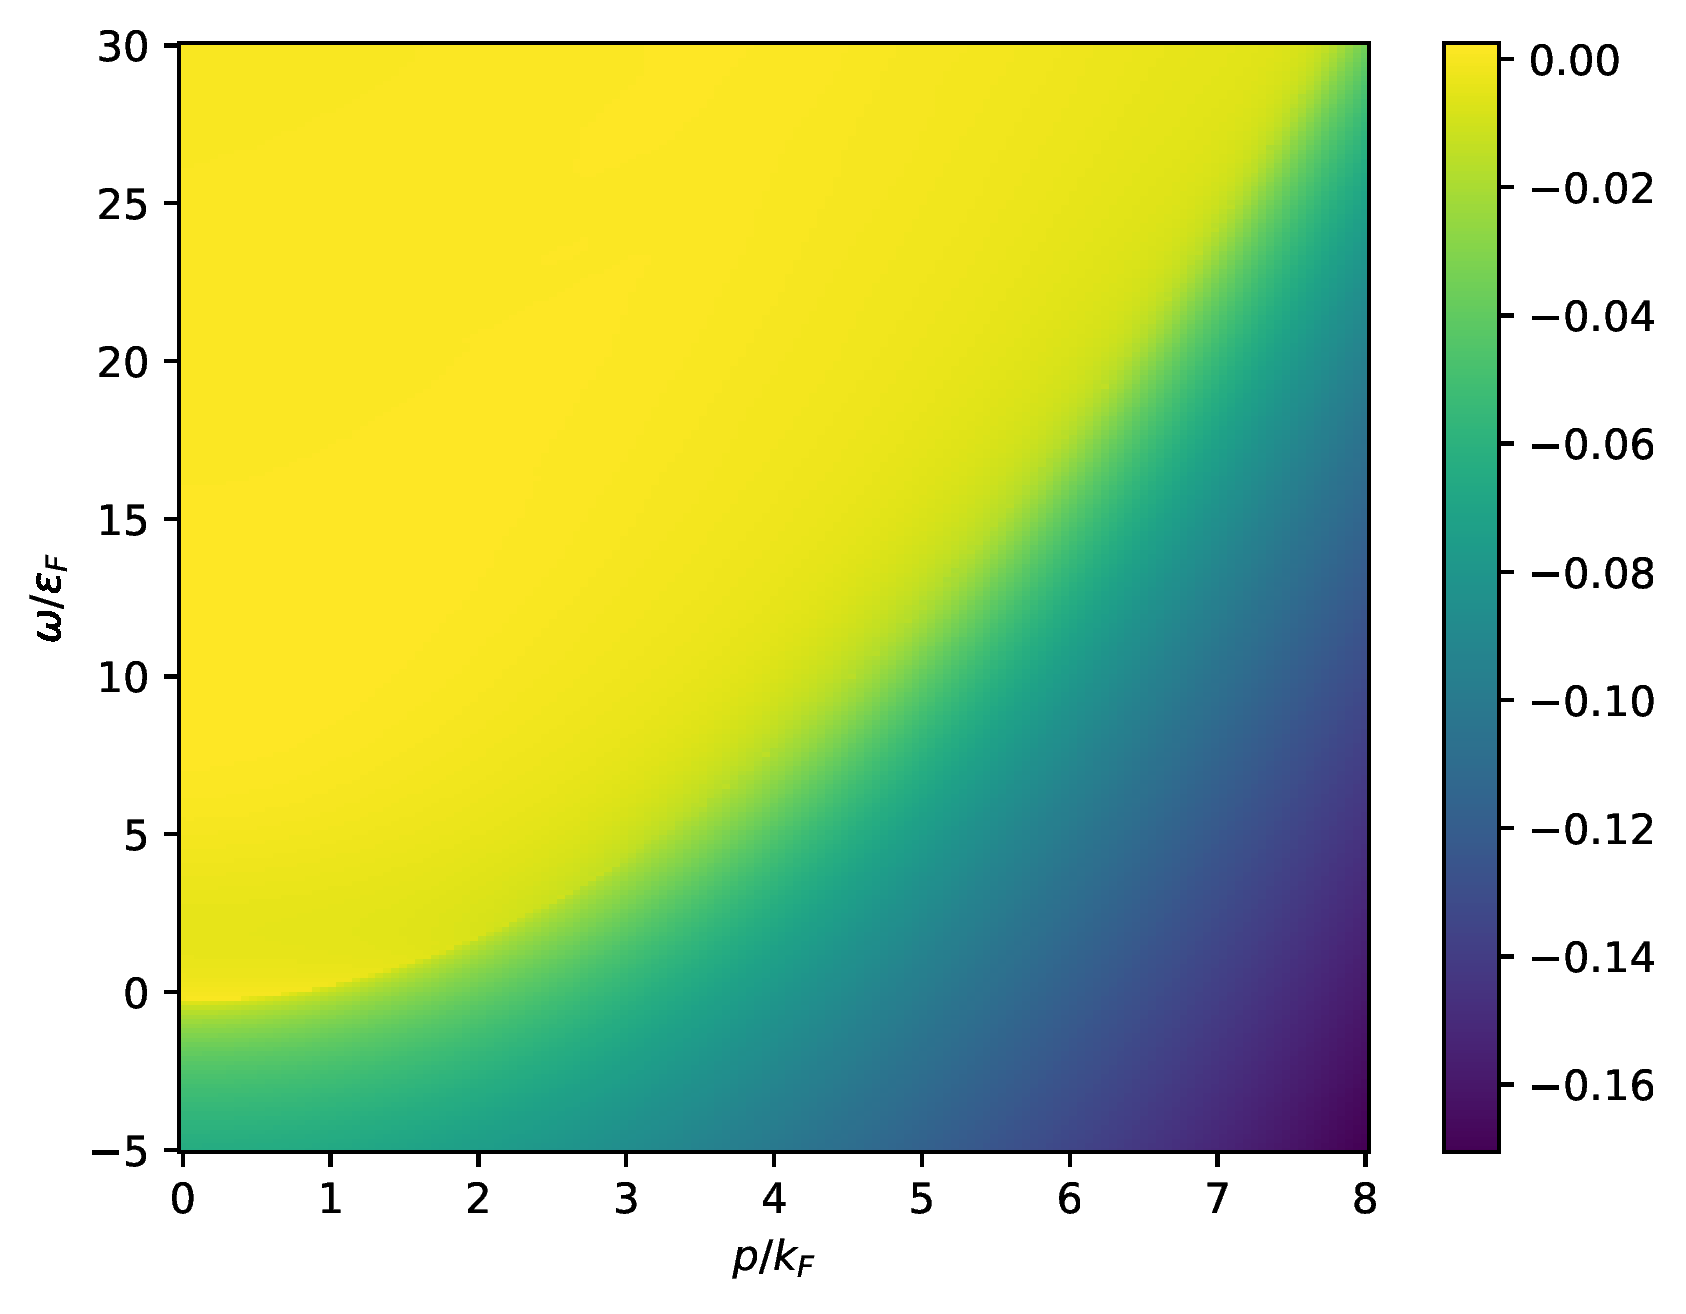
\includegraphics[width=0.475\textwidth]{figs/boson_self_re.png}}
	\subfigure[$\text{Im}\,\Pi^{R}_{\phi}(\omega,\bm{p})$]{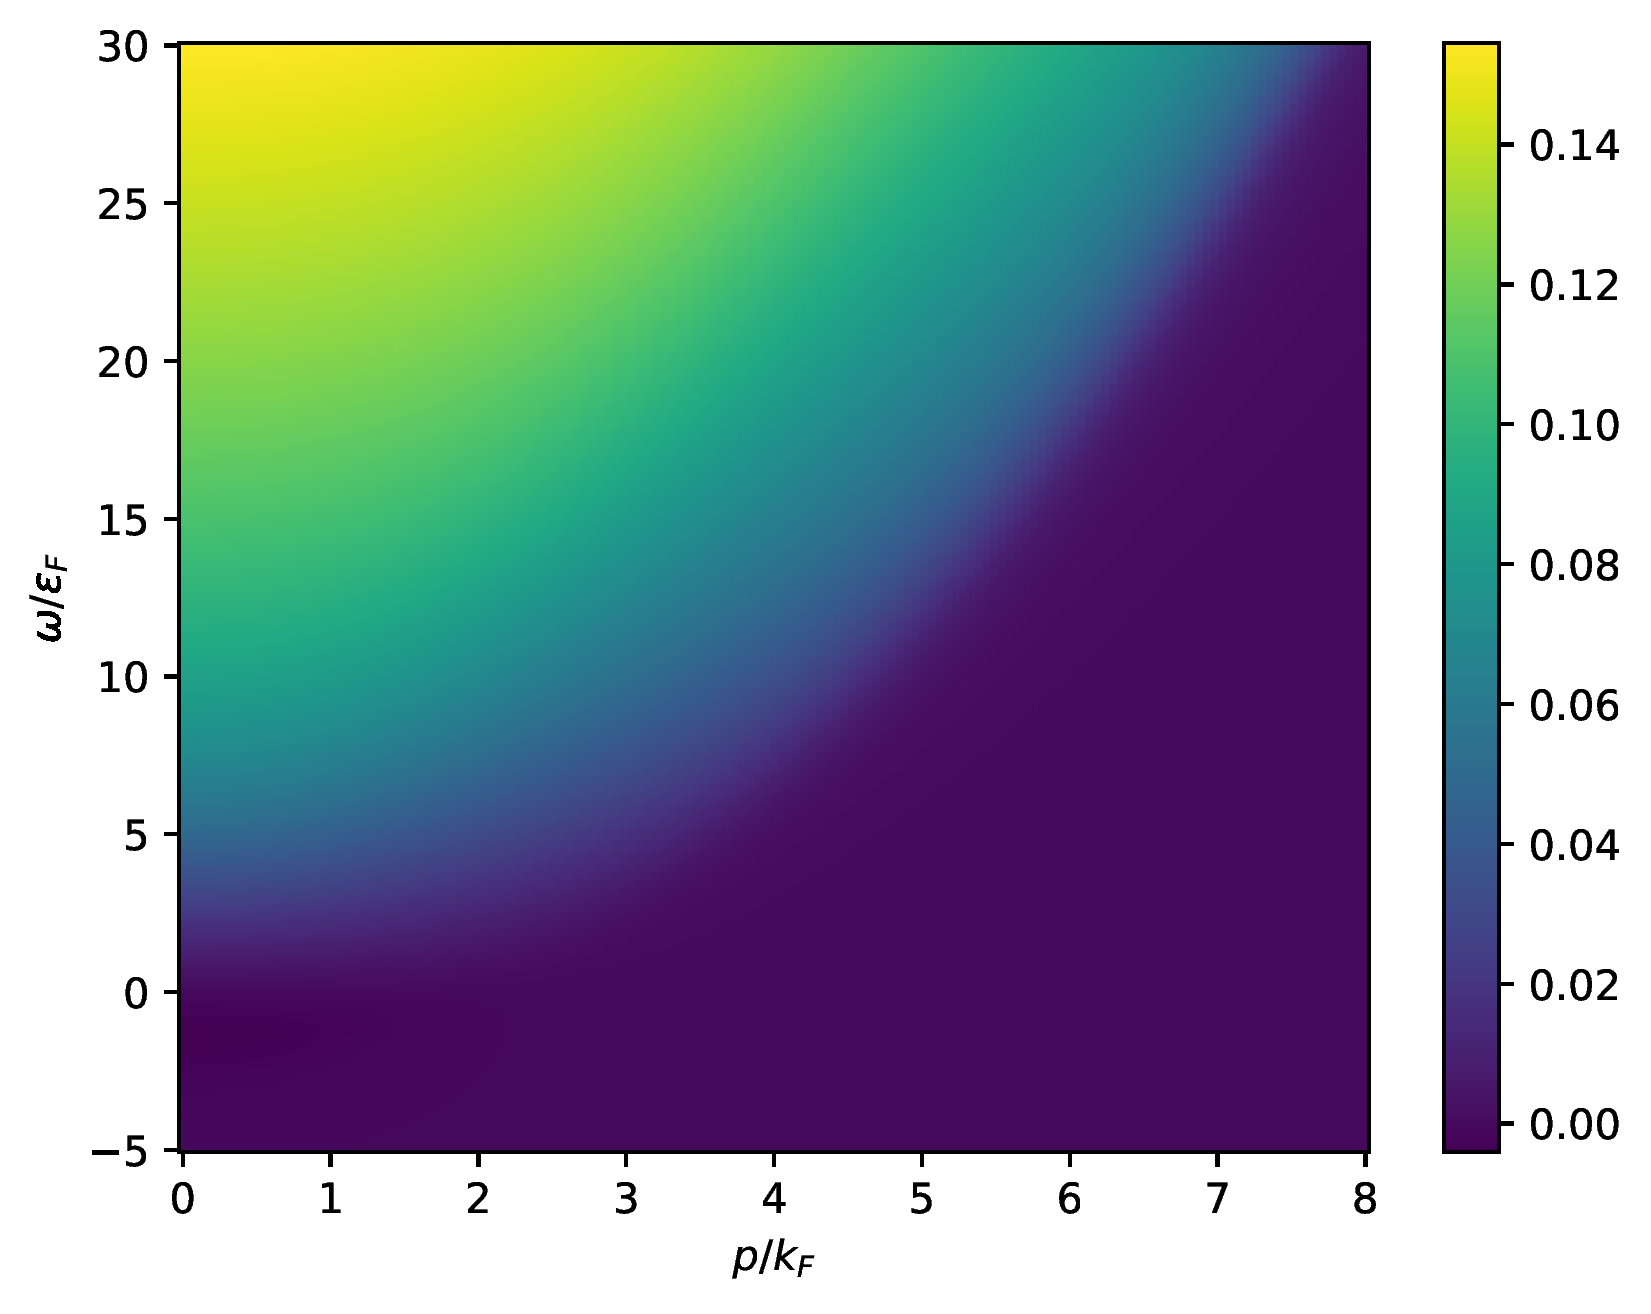
\includegraphics[width=0.47\textwidth]{figs/boson_self_im.png}}
	\caption[Boson self-energy]{Real and imaginary part of the retarded boson self-energy $\Pi^{R}_{\phi}(\omega,\bm{p})$.}
	\label{fig:boson-self-energy}
\end{figure*}


\clearpage

%%%%%%%%%%%%%%%%%%%%%%%%%%%%
\section{Fermion self-energy calculation}
\label{app:fermion-self-energy-calculation}


For the fermion self-energy, there are no analytical results for the non-selfconsistent case in the single-channel model, since the bare boson propagator has no dispersion. Therefore, the self-energy has to be computed numerically from the spectral functions. The general expression for the retarded fermion self-energy $\Sigma^R_{\psi}(\omega,\bm{p})$ is
%
\begin{align}
	\label{eq:ferm_self}
	\Sigma^R_{\psi}(\omega,\bm{p}) = -h^2\int_{\bm{q},\lambda_1,\lambda_2} \rho_{\phi}(\lambda_1,\bm{q}) \rho_{\psi}(\lambda_2,\bm{p}-\bm{q})\, \frac{n_B(\lambda_1)+n_F(\lambda_2)}{-\omega+\lambda_1-\lambda_2-i0^+} \,,
\end{align}
%
Taking the imaginary part recovers Eq.~\eqref{eq:imaginary-part-self-energies}. Note that the imaginary part is strictly negative, since all quantities are positive definite, except of $n_B(\lambda_1)$ and $\rho_{\phi}(\lambda_1)$. Fortunately, the sign change of the boson distribution and spectral function occurs both at $\lambda_1=0$, and $n_B(\lambda_1),\rho_{\phi}(\lambda_1)<0$ for $\lambda_1<0$. Moreover, the pole of $n_B(\lambda_1)$ at $\lambda_1=0$ is exactly canceled by the zero crossing of the boson spectral function $\rho_{\phi}(\lambda_1)$, see Section~\ref{section:spectral-representation}. Thus, the imaginary part of Eq.~\eqref{eq:ferm_self} is a regular expression that can be evaluated numerically. The only difficulty is the highly peaked structure of the integrand, and will be discussed in the numerical Appendix~\ref{app:numerical-implementation}.

As a side remark, we note that non-selfconsistent results for the fermion self-energy can be derived for the two-channel model with dynamic bosons. Inserting the classical spectral functions $\rho_{\psi}(\lambda,\bm{p})=\delta(\lambda-\bm{p}^2+\mu)$ and $\rho_{\phi}(\lambda,\bm{p})=\delta(\lambda-\bm{p}^2/2-\nu+2\mu)$, we obtain
\begin{align}
\Sigma^R_{\psi}(\omega, \bm{p}) = -h^2 \int_{\bm{q}} \frac{n_B(\varepsilon_{\bm{q}}/2+\nu-2\mu) + n_F(\varepsilon_{\bm{p-q}}-\mu)}{-\omega+\varepsilon_{\bm{q}}/2- \varepsilon_{\bm{p-q}}+\nu-\mu-i0^+} \,.
\end{align}
However, this will not be evaluated further in this work. \\

Fig.~\ref{fig:fermion-self-energy} shows an example for the real and imaginary part of the retarded fermion self-energy $\Sigma^{R}_{\psi}(\omega,\bm{p})$ for the balanced case at unitarity and $\beta\mu=0.13146$.

\vspace{1cm}

\begin{figure*}[h]
	\centering
	\subfigure[$\text{Re}\,\Sigma^{R}_{\psi}(\omega,\bm{p})$]{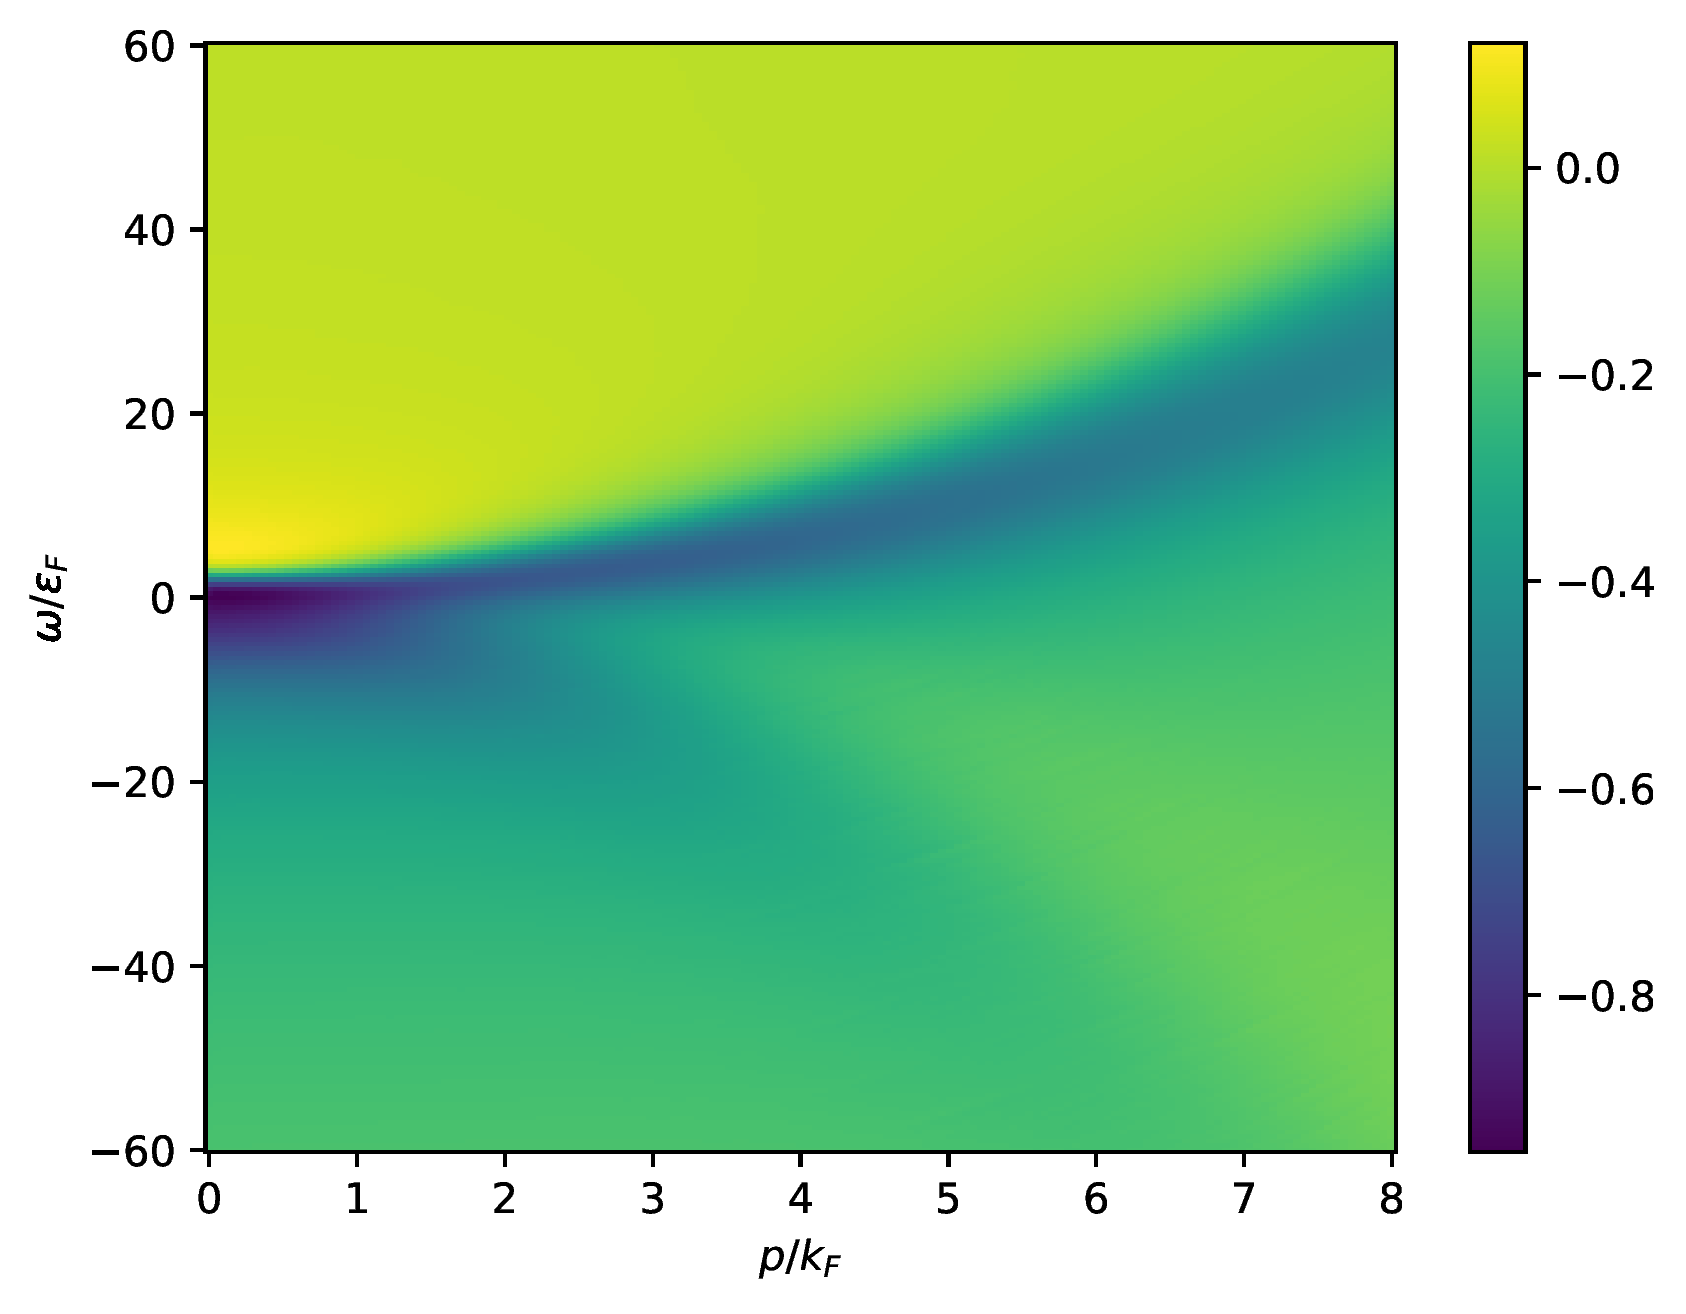
\includegraphics[width=0.47\textwidth]{figs/fermion_self_re.png}}
	\subfigure[$\text{Im}\,\Sigma^{R}_{\psi}(\omega,\bm{p})$]{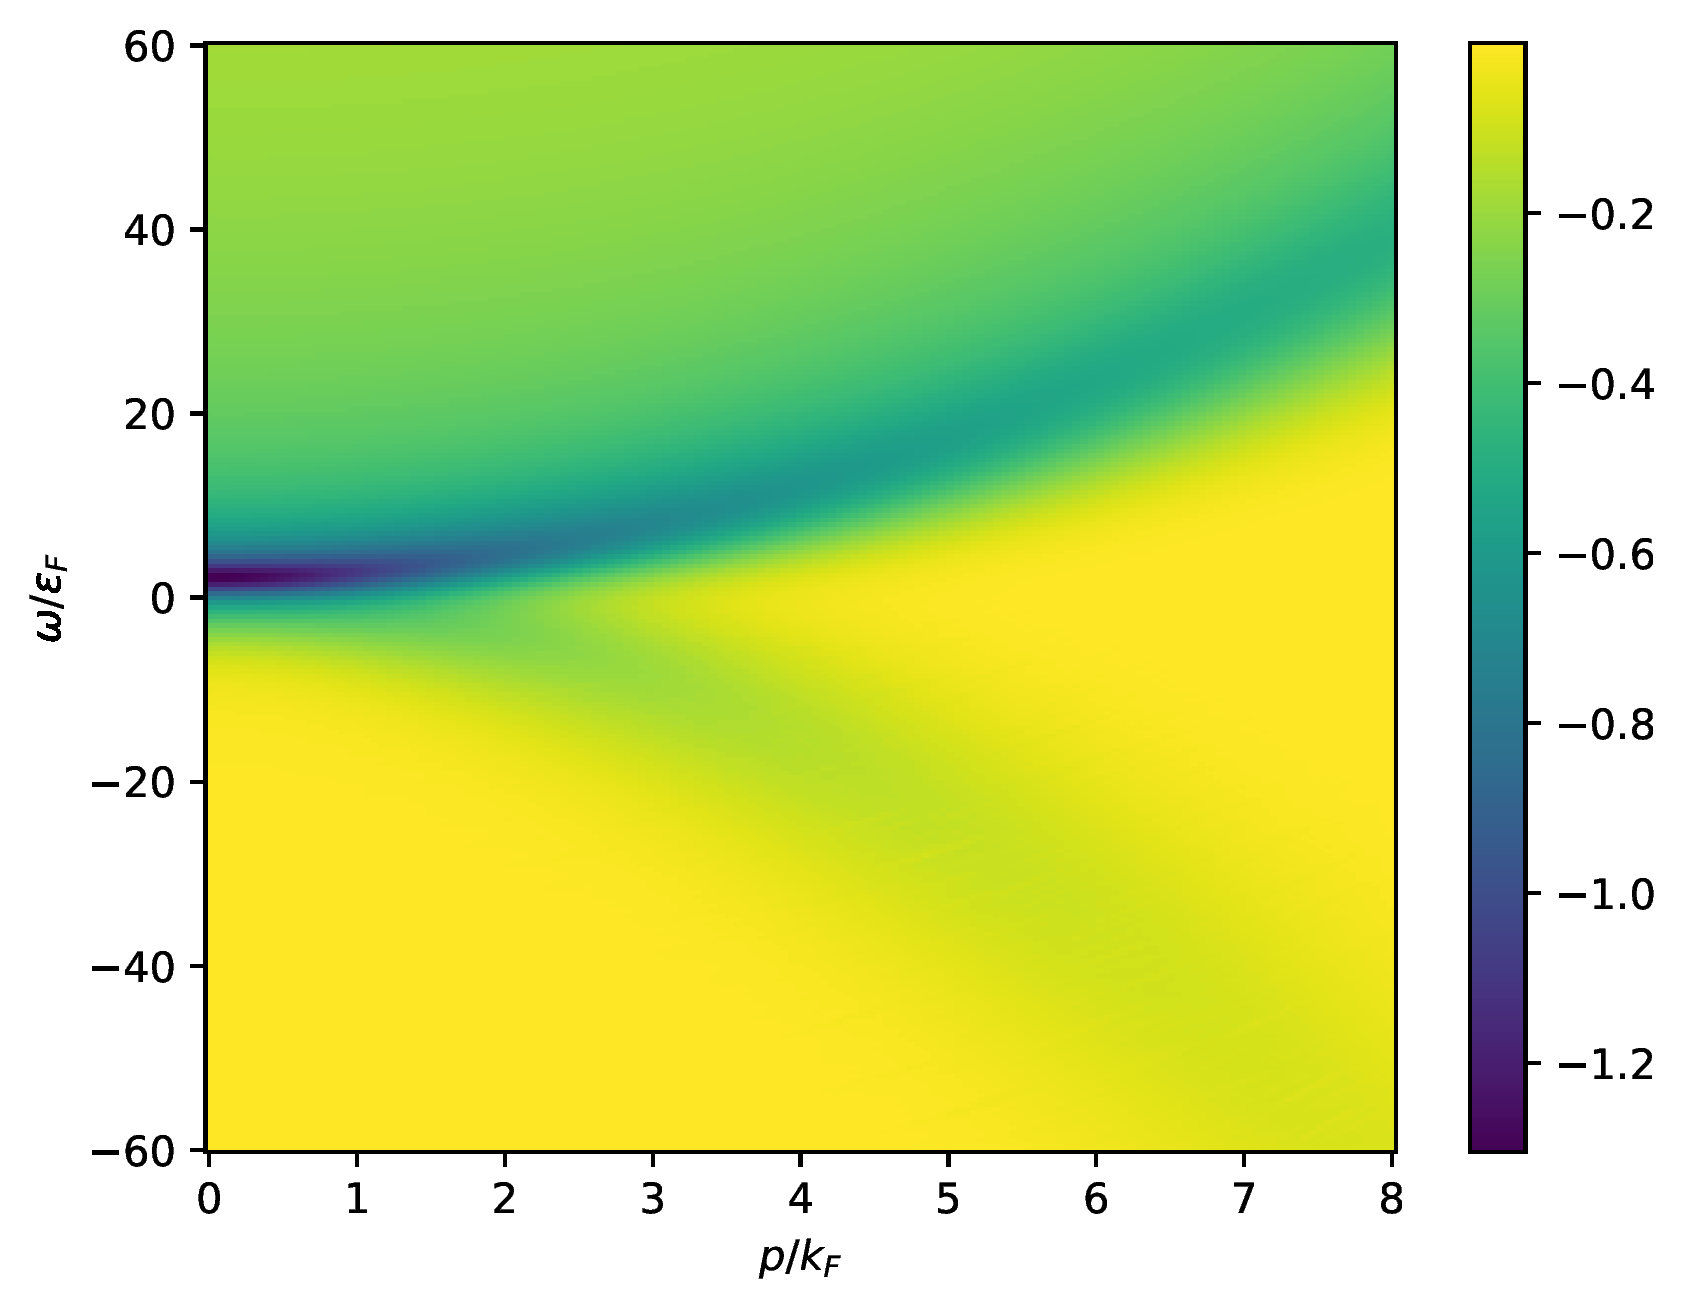
\includegraphics[width=0.47\textwidth]{figs/fermion_self_im.png}}
	\caption[Fermion self-energy]{Real and imaginary part of the retarded fermion self-energy $\Sigma^{R}_{\psi}(\omega,\bm{p})$.}
	\label{fig:fermion-self-energy}
\end{figure*}